\section{Introduction}

Dynamic manipulation and management of linear deformable objects such as ropes, chains, vacuum cords, charger cables, power cables, tethers, and dog leashes are common in daily life. For example, a person vacuuming may find that the vacuum power cable is stuck on a chair, and use dynamic manipulation to ``vault'' the cable over the chair. If the first motion does not succeed, the human can try again, adapting their motion to the failure.  In this paper, we explore how a robot can teach itself to perform three tasks:

\begin{description}[align=left,leftmargin=0pt]
    \item[Task 1: Vaulting] The robot dynamically manipulates a cable to move from one side of an obstacle to another. %A success is when the rope lands on the other side of the obstacle, and a failure is when the rope remains on the same side of the obstacle, or lands on top of it.
    %% I think these measures of success are somewhat implied here, and should be discussed in detail in the experiments. -JI 
    \item[Task 2: Knocking] The robot dynamically manipulates a cable to knock a target object off an obstacle. %A success is when the rope knocks the target so it moves in any way, and a failure is when the target stays stationary.
    %% I think these measures of success are somewhat implied here, and should be discussed in detail in the experiments. -JI 
    \item[Task 3: Weaving] The robot dynamically manipulates a cable to weave it between three obstacles. %A success is when the cable forms an interweaving shape between the obstacles, and a failure is any other case.
    % \item \textbf{Task 4: Twirling. } Whip the rope in a jump-rope pattern. \harry{TODO: Finalize. Will get it done by the end of this week.}
\end{description} 

% \begin{figure}[t]
\vspace*{5pt}

\center
%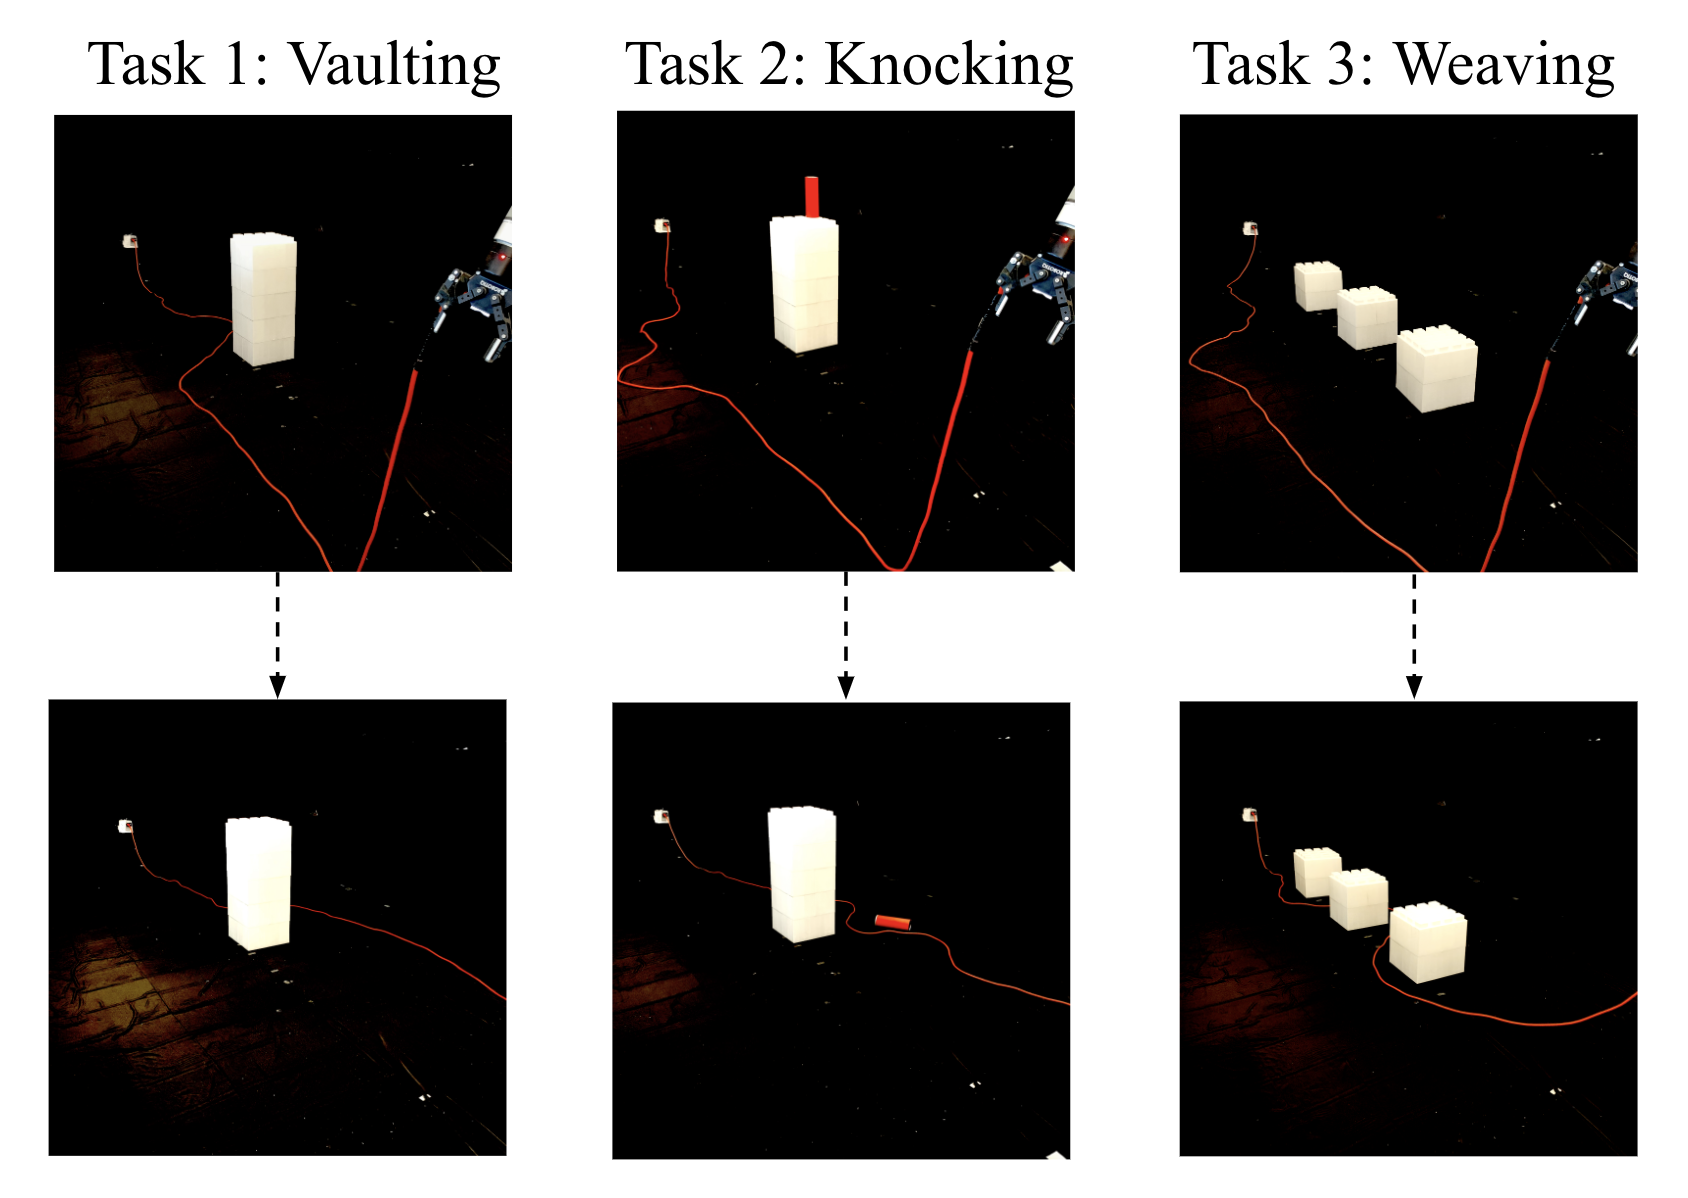
\includegraphics[width=0.48\textwidth]{figures/teaser1.png}
\begin{tikzpicture}[
every node/.style={outer sep=0,node distance=0pt,inner sep=0},
arr/.style={-latex,line width=1pt}]
% IEEE conference format: column width = 3.4in = 244.8pt
% 3 pictures * 80pt = 240pt
% (244.8 - 240)/2 = 4.8/2 = 2.4pt = spacing between pictures
% \node [options] (name) {LaTex Contents of Node};


% \draw [-Triangle,thick] (from_name) -- (to_name); 
% "-Latex" and "-triangle" are arrow types
\node (vs) {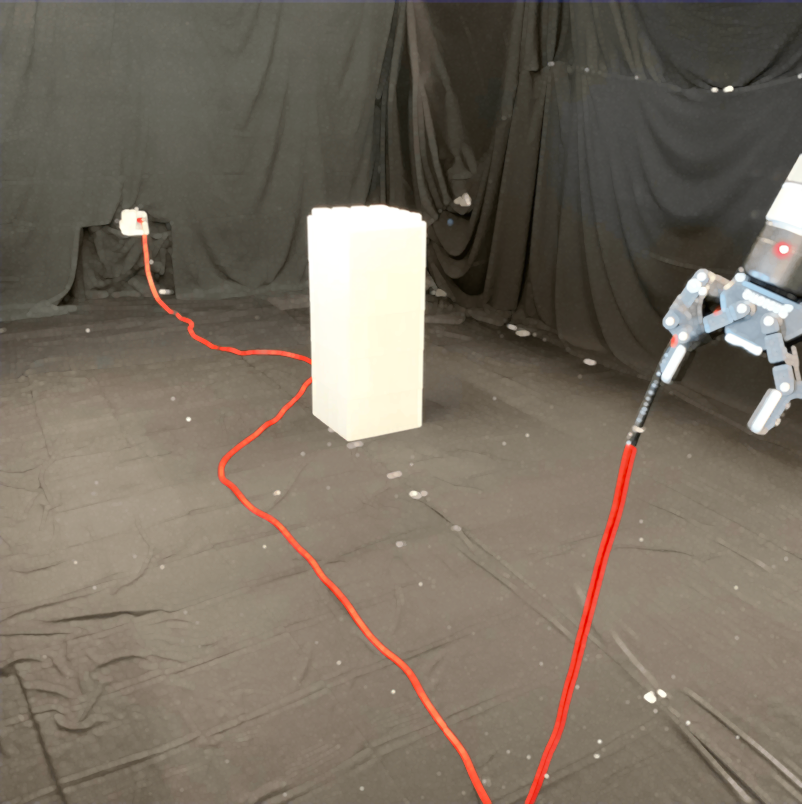
\includegraphics[width=80pt]{figures/teaser_vaulting_start.png}};
\node [right=2.4pt of vs] (ks) {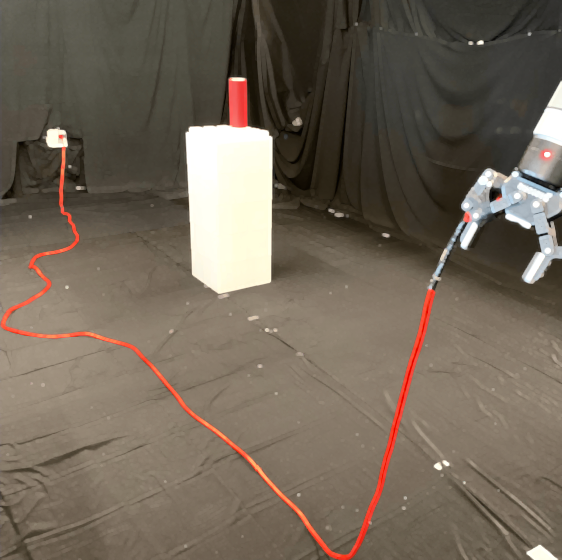
\includegraphics[width=80pt]{figures/teaser_knocking_start.png}};
\node [right=2.4pt of ks] (ws) {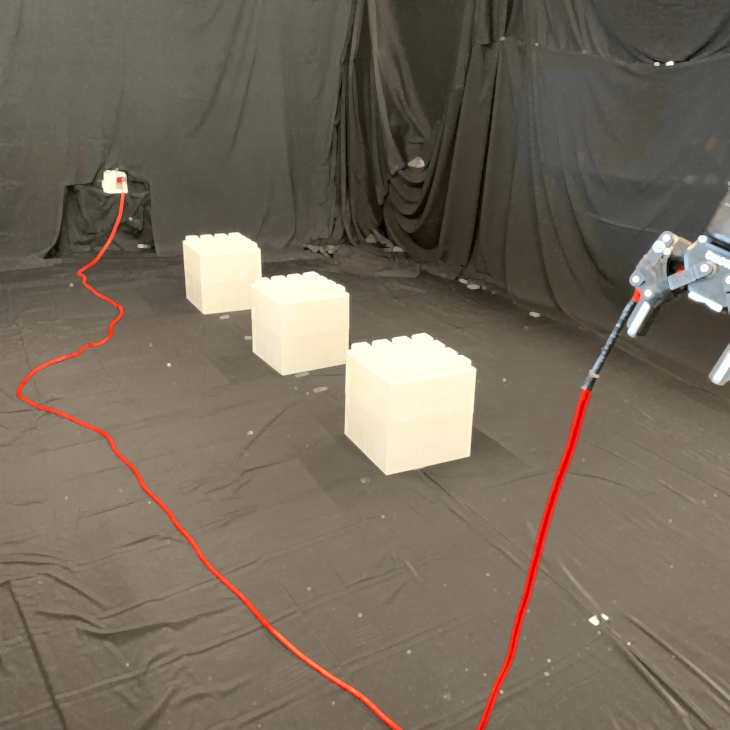
\includegraphics[width=80pt]{figures/teaser_weaving_start.png}};
\node [below=12pt of vs] (ve) {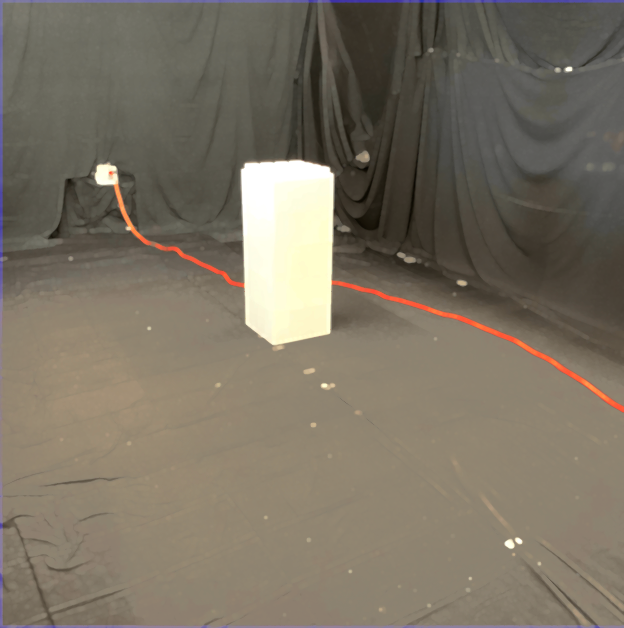
\includegraphics[width=80pt]{figures/teaser_vaulting_end.png}};
\node [below=12pt of ks] (ke) {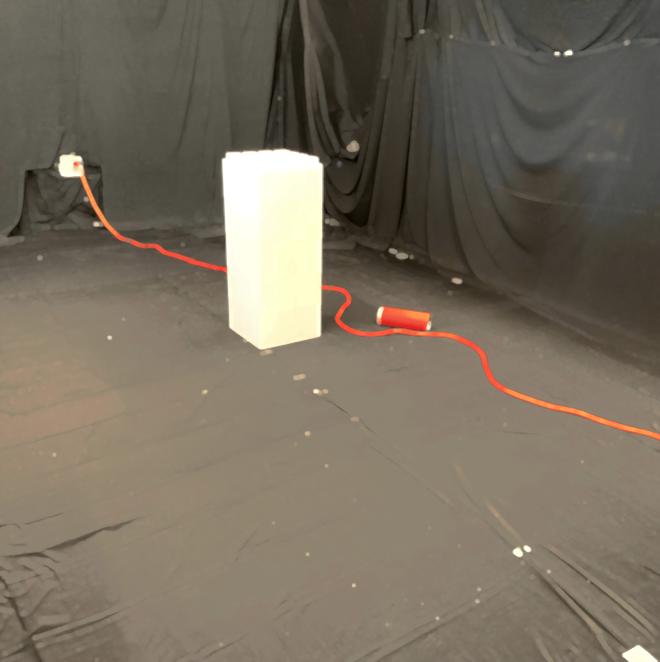
\includegraphics[width=80pt]{figures/teaser_knocking_end.png}};
\node [below=12pt of ws] (we) {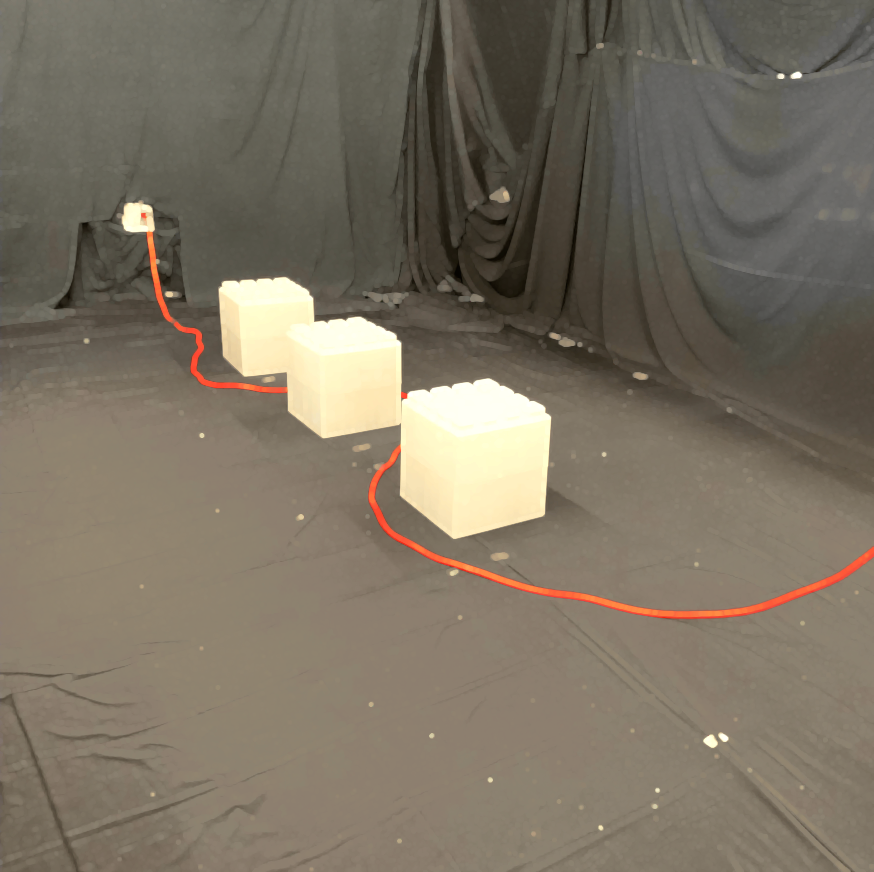
\includegraphics[width=80pt]{figures/teaser_weaving_end.png}};
\draw [arr] (vs) -- (ve);
\draw [arr] (ks) -- (ke);
\draw [arr] (ws) -- (we);
\node [below=4pt of ve] {\footnotesize (a) Task 1: Vaulting};
\node [below=4pt of ke] {\footnotesize (b) Task 2: Knocking};
\node [below=4pt of we] {\footnotesize (c) Task 3: Weaving};
\end{tikzpicture}
\caption{
\small
Illustration of the 3 tasks: Vaulting, Knocking, and Weaving in real experiments with an orange 18-gauge cable. %The cable is plugged into the wall on one end, and attached to the robot's gripper on the other end.
}
\vspace*{-15pt}
\label{fig:three_tasks}
\end{figure}
To accomplish these tasks, we propose to generate trajectories using a parameterized function. To reduce the complexity of parameterizing actions, we compute minimum-jerk trajectories using DJ-GOMP~\cite{GOMP, DJGOMP} that take as input the apex point in the trajectory.  This point, combined with task-specific starting and ending arm configurations, are used to generate a single high-speed trajectory for a physical UR5 robot. 
\begin{figure}
    \centering
    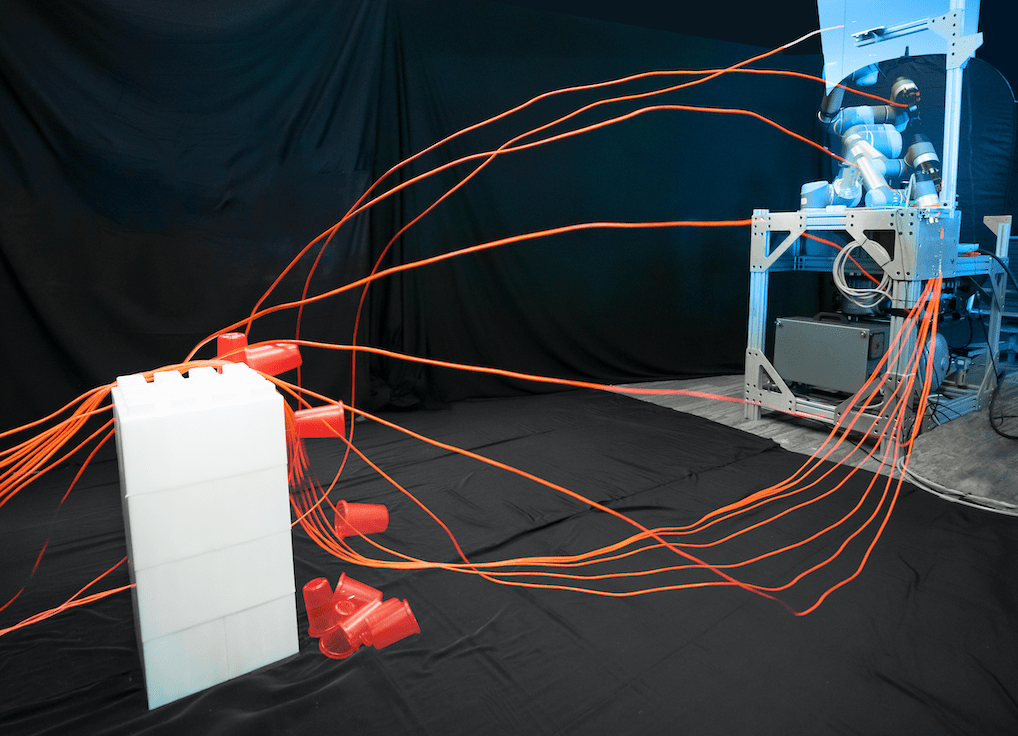
\includegraphics[width=\linewidth]{figures/teaser_new1.png}
    \caption{Long exposure photo of a UR5 robot dynamically manipulating an orange cable fixed at one end (far left) to knock the red target cup off the white obstacle using the learned 3d apex point and minimum-jerk robot trajectory.}
    \label{fig:teaser_new}
    \vspace*{-20pt}
\end{figure}
We present a self-supervised deep imitation learning pipeline that learns to predict the apex point given target positions. Using a simulator we develop for vaulting, with a simulated UR5, we obtain an example action that completes the vaulting task. For any of the three tasks in the real world (see Fig.~\ref{fig:teaser_new}), we then have the physical UR5 continually execute actions based on the action computed in simulation, with noise added to increase dataset diversity. While the robot performs actions, one end of the cable is attached to its gripper, and the other is fixed to a wall. (Hereafter, we use \emph{cable} to refer to any 1D deformable object with low stiffness, such as ropes, cords, and strings.) This process results in a self-supervised procedure for collecting a large dataset. We use the resulting data to train a deep neural network policy to predict an action (i.e., the apex point) given a target position. %The physical experiments setup is shown in Fig.\ref{fig:teaser_new}.
%The system learns using physical trials on a UR5 robot. 

This paper contributes:
\begin{enumerate}
    \item Three novel dynamic cable manipulation tasks: vaulting, knocking, and weaving.
    \item INDy, a self-supervised framework for collecting data and learning a dynamic manipulation policy using parameterized minimum-jerk trajectories.
    \item A simulation platform to experiment with novel tasks and policy learning.
    \item Physical experiments evaluating the policies with a UR5 robot on 5 different cables.
\end{enumerate}


%While humans often accomplish such motions, it is difficult for a robot to generate a feasible trajectory to accomplish this task.
% The key notion we tackle in this paper making the rope manipulation dynamic---with few swift motions of a its manipulator arm a robot accomplishes a task.  We contrast this to prior work that explored quasi-static manipulation of cables in a 2D space, such as knot-tying~\cite{knot_planning_2003, nair_rope_2017}, shape-matching~\cite{nair_rope_2017,yan2020learning} and untangling~\cite{rope_untangling_2013,grannen2020untangling}, few attempt to manipulate cables dynamically in a full 3D space. \jeffi{TODO: reword to place dynamic manipulation in context.}
%To reduce increase the repeatability of actions, we reset the cable each time by pulling it taut and slowing dropping it before each dynamic motion.
%and does not explicitly model cable dynamics (see Section~\ref{sec:method} for details). To minimize the damage to the robot, we generate a trajectory defined by those three points (start, learned 3D apex point, and end) with minimal jerk.
